\documentclass[twoside,a4paper]{article}
\usepackage{geometry}
\geometry{margin=1.5cm, vmargin={0pt,1cm}}
\setlength{\topmargin}{-1cm}
\setlength{\paperheight}{29.7cm}
\setlength{\textheight}{25.3cm}

% useful packages.
\usepackage{amsfonts}
\usepackage{amsmath}
\usepackage{amssymb}
\usepackage{amsthm}
\usepackage{enumerate}
\usepackage{graphicx}
\usepackage{multicol}
\usepackage{fancyhdr}
\usepackage{layout}
\usepackage{listings}
\usepackage{float, caption}

\lstset{
    basicstyle=\ttfamily, basewidth=0.5em
}

% some common command
\newcommand{\dif}{\mathrm{d}}
\newcommand{\avg}[1]{\left\langle #1 \right\rangle}
\newcommand{\difFrac}[2]{\frac{\dif #1}{\dif #2}}
\newcommand{\pdfFrac}[2]{\frac{\partial #1}{\partial #2}}
\newcommand{\OFL}{\mathrm{OFL}}
\newcommand{\UFL}{\mathrm{UFL}}
\newcommand{\fl}{\mathrm{fl}}
\newcommand{\op}{\odot}
\newcommand{\Eabs}{E_{\mathrm{abs}}}
\newcommand{\Erel}{E_{\mathrm{rel}}}

\begin{document}

\pagestyle{fancy}
\fancyhead{}
\lhead{Wenchong Huang (3200100006)}
\chead{Numerical PDE homework \#2}
\rhead{Apr.1st, 2023}


\section*{I. Exercise 9.5 (Prove Theorem 9.4.)}

\;\;\;\;\;\;Actually we want to prove the following two inequalities:
\begin{equation}
    \frac{||\mathbf{r}||_2\cdot||\mathbf{x}||_2}{||A||_2\cdot||A^{-1}||_2\cdot||\mathbf{b}||_2\cdot||\mathbf{e}||_2}\leq 1 \quad \text{and} \quad
    \frac{||\mathbf{b}||_2\cdot||\mathbf{e}||_2}{||A||_2\cdot||A^{-1}||_2\cdot||\mathbf{r}||_2\cdot||\mathbf{x}||_2}\leq 1
\end{equation}

We have $||A^{-1}||_2\cdot ||\mathbf{b}||\geq ||A^{-1}\mathbf{b}||_2=||\mathbf{x}||_2$ and $||A||_2\cdot ||\mathbf{e}||\geq ||A\mathbf{e}||_2=||\mathbf{r}||_2$. Hence for the first inequality:
\begin{equation*}
    \frac{||\mathbf{r}||_2\cdot||\mathbf{x}||_2}{||A||_2\cdot||A^{-1}||_2\cdot||\mathbf{b}||_2\cdot||\mathbf{e}||_2}\leq \frac{||\mathbf{r}||_2\cdot||\mathbf{x}||_2}{||\mathbf{x}||_2\cdot||\mathbf{r}||_2} = 1
\end{equation*}

Also, $||A^{-1}||_2\cdot ||\mathbf{r}||\geq ||A^{-1}\mathbf{r}||_2=||\mathbf{e}||_2$ and $||A||_2\cdot ||\mathbf{x}||\geq ||A\mathbf{x}||_2=||\mathbf{b}||_2$. Hence for the second inequality:
\begin{equation*}
    \frac{||\mathbf{b}||_2\cdot||\mathbf{e}||_2}{||A||_2\cdot||A^{-1}||_2\cdot||\mathbf{r}||_2\cdot||\mathbf{x}||_2}\leq \frac{||\mathbf{b}||_2\cdot||\mathbf{e}||_2}{||\mathbf{e}||_2\cdot||\mathbf{b}||_2} = 1
\end{equation*}

Hence Theorem 9.4 is proved.

\section*{II. Exercise 9.8 (Compute $\text{cond}(A)$ for $n=8$ and $n=1024$.)}

\;\;\;\;\;\;We konw $\lambda_k(A)=4n^2\sin^2\frac{k\pi}{2n}$ for $k=1,2,...,n-1$. Since $A$ is symmetric, we got $||A||_2$ immediately by
\begin{equation*}
    ||A||_2=\max \sqrt{\lambda(A^TA)} = \max|\lambda(A)| = 4n^2\sin^2\frac{(n-1)\pi}{2n}.
\end{equation*}

Since $\lambda_k(A^{-1})=\lambda_k(A)^{-1}$, we can also got $||A^{-1}||_2$ by
\begin{equation*}
    ||A^{-1}||_2=\min|\lambda(A)^{-1}| = \frac{1}{4n^2\sin^2\frac{\pi}{2n}}.
\end{equation*}

It follows that
\begin{equation*}
    \text{cond}(A) = ||A||_2\cdot ||A^{-1}||_2=\frac{\sin^2\frac{(n-1)\pi}{2n}}{\sin^2\frac{\pi}{2n}}.
\end{equation*}

Use a calculator to compute the value for $n=8$ and $n=1024$, we got
\begin{equation*}
    \text{cond}(A)|_{n=8}\approx 48.99 \quad \text{and} \quad \text{cond}(A)|_{n=1024}\approx 1.046\times 10^6.
\end{equation*}

\section*{III. Exercise 9.11 (Show the maximum wavenumber representable on $\Omega^h$.)}

\;\;\;\;\;\;$n_\text{max}$ reaches when we alternate from local maximum and local minumum at the $n+1$ grid points. As the following figure shows.

\begin{figure}[H]
    \centering
    \begin{minipage}[t]{0.42\textwidth}
        \centering
        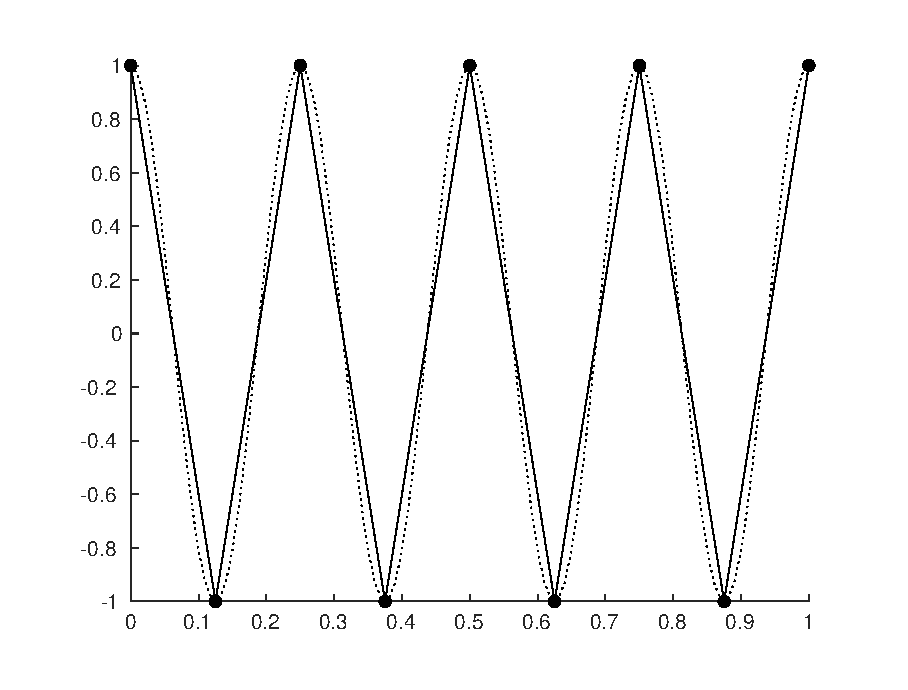
\includegraphics[width=0.95\textwidth]{figure/ex9_11_1.eps}
        \caption*{$n_\text{max}=\frac{1}{h}$}
    \end{minipage}
    \begin{minipage}[t]{0.42\textwidth}
        \centering
        \includegraphics[width=0.95\textwidth]{figure/ex9_11_2.eps}
    \end{minipage}
\end{figure}

We can see $n_\text{max}=\frac{1}{h}$. When we require the Fourier mode be $0$ at the bondary points, the maximum number of alternation between local extrema is reduced by one. Hence in this condition, we have $n_\text{max}=\frac{1}{h}-1$.

\section*{IV. Exercise 9.14 (Plot the case of $n=6$ for Example 9.13.)}

\;\;\;\;\;\;As the following figure shows.
\begin{figure}[H]
    \centering
    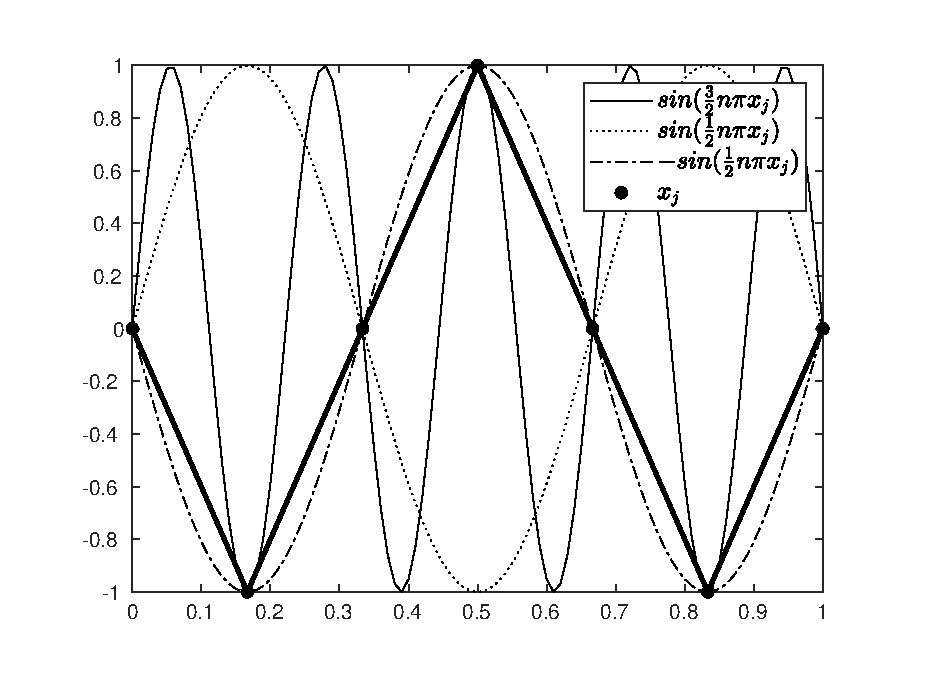
\includegraphics[width=0.4\textwidth]{figure/ex9_14.eps}
    \caption{The case of $n=6$ for Example 9.13.}
\end{figure}

\section*{V. Exercise 9.17 (Prove Lemma 9.16.)}
\;\;\;\;\;\;For the $k$th eigenvalue $\lambda_k$ and the corresponding eigenvector $\mathbf{w}_k$ we have:
\begin{equation*}
    (\lambda_k\mathbf{w}_k)_j = \left(1-2\omega\sin^2\frac{k\pi}{2n}\right)\sin\frac{jk\pi}{n}=\left(1-\omega+\omega\cos\frac{k\pi}{n}\right)\sin\frac{jk\pi}{n}
\end{equation*}

Now,
\begin{equation*}
    (T_\omega\mathbf{w}_k)_1=(1-\omega)\sin\frac{k\pi}{n}+\frac{\omega}{2}\sin\frac{2k\pi}{n}=\left(1-\omega+\omega\cos\frac{k\pi}{n}\right)\sin\frac{k\pi}{n}=(\lambda_k\mathbf{w}_k)_1.
\end{equation*}

And for each $2\leq j\leq n-2$, we have
\begin{align*}
    (T_\omega\mathbf{w}_k)_j &= (1-\omega)\sin\frac{jk\pi}{n}+\frac{\omega}{2}\left(\sin\frac{(j-1)k\pi}{n}+\sin\frac{(j+1)k\pi}{n}\right)\\
    &= (1-\omega)\sin\frac{jk\pi}{n}+\frac{\omega}{2}\left(\sin\frac{jk\pi}{n}\cos\frac{k\pi}{n}-\cos\frac{jk\pi}{n}\sin\frac{k\pi}{n}+\sin\frac{jk\pi}{n}\cos\frac{k\pi}{n}+\cos\frac{jk\pi}{n}\sin\frac{k\pi}{n}\right)\\
    &= (1-\omega)\sin\frac{jk\pi}{n}+\omega\sin\frac{jk\pi}{n}\cos\frac{k\pi}{n}=(\lambda_k\mathbf{w}_k)_j.
\end{align*}

Note that
\begin{equation*}
    \sin\frac{(n-1)k\pi}{n}\cos\frac{k\pi}{n}+\cos\frac{(n-1)k\pi}{n}\sin\frac{k\pi}{n} = \sin(k\pi) = 0
\end{equation*}

Then finally we have
\begin{align*}
    (T_\omega\mathbf{w}_k)_{n-1} &= (1-\omega)\sin\frac{(n-1)k\pi}{n}+\frac{\omega}{2}\sin\frac{(n-2)k\pi}{n}\\
    &= (1-\omega)\sin\frac{(n-1)k\pi}{n}+\frac{\omega}{2}\left(\sin\frac{(n-1)k\pi}{n}\cos\frac{k\pi}{n}-\cos\frac{(n-1)k\pi}{n}\sin\frac{k\pi}{n}\right)\\
    &= (1-\omega)\sin\frac{(n-1)k\pi}{n}+\frac{\omega}{2}\left(\sin\frac{(n-1)k\pi}{n}\cos\frac{k\pi}{n}+\sin\frac{(n-1)k\pi}{n}\cos\frac{k\pi}{n}\right)\\
    &= (1-\omega)\sin\frac{(n-1)k\pi}{n}+\omega\sin\frac{(n-1)k\pi}{n}\cos\frac{k\pi}{n} = (\lambda_k\mathbf{w}_k)_{n-1}.
\end{align*}

And hence $T_\omega\mathbf{w}_k=\lambda_k\mathbf{w}_k$. Then Lemma 9.16 is proved.

\section*{VI. Exercise 9.18 (Reproduce Fig. 2.7 and show slow convergence.)}
\;\;\;\;\;\;Reproduce Fig. 2.7 in the book by Briggs et al.[2000] as following.
\begin{figure}[H]
    \centering
    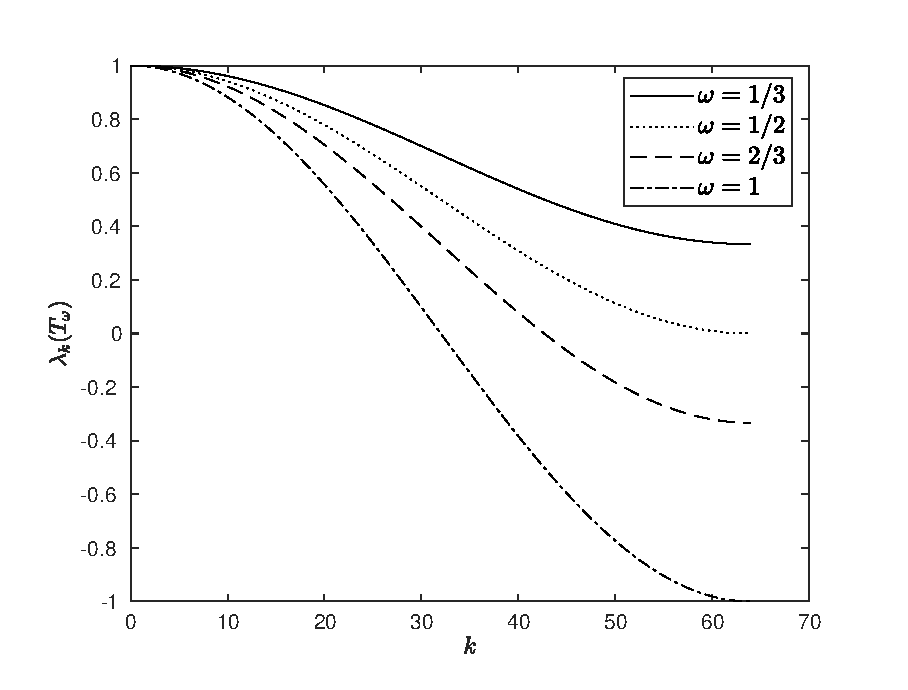
\includegraphics[width=0.4\textwidth]{figure/ex9_18.eps}
    \caption{Reproduce Fig. 2.7 in the book by Briggs et al.[2000].}
\end{figure}

It was produced by the following \textbf{matlab} code.
\begin{lstlisting}
    w = [1/3, 1/2, 2/3, 1];
    lstl = ['k', ':k', '--k', '-.k'];
    ind = [1,1,2,3,4,6,7,9];
    n = 64;
    rho = zeros(1,4);
    for wk = 1:4
        cw = w(wk);
        k = 0:0.1:n;
        lam = 1-2*cw*sin(k*pi/(2*n)).^2;
        rho(wk) = lam(11);
        plot(k,lam,lstl(ind(2*wk-1):ind(2*wk)))
        hold on
    end
    disp(rho);
    xlabel('$k$','interpreter','latex');
    ylabel('$\lambda_k(T_\omega)$','interpreter','latex');
    legend('$\omega=1/3$','$\omega=1/2$','$\omega=2/3$','$\omega=1$','interpreter','latex',
'FontSize',12);
\end{lstlisting}

Clearly $\rho(T_{\omega_1})>\rho(T_{\omega_2})$ for any $\omega_1<\omega_2$. Then
\begin{equation*}
    \rho(T_\omega)\geq \rho(T_1)\approx 0.998795> 0.9986 \quad \text{for all } \omega\in[0,1].
\end{equation*}

And hence slow convergence.

\section*{VII. Exercise 9.21 (Reproduce Fig. 2.8.)}
\;\;\;\;\;\;Reproduce Fig. 2.8 in the book by Briggs et al.[2000] as following.
\begin{figure}[H]
    \centering
    \begin{minipage}[t]{0.33\textwidth}
        \centering
        \includegraphics[width=0.95\textwidth]{figure/ex9_21_1.eps}
        \caption*{$\omega=1$ (Regular Jacobi)}
    \end{minipage}
    \begin{minipage}[t]{0.33\textwidth}
        \centering
        \includegraphics[width=0.95\textwidth]{figure/ex9_21_2.eps}
        \caption*{$\omega=\frac{2}{3}$}
    \end{minipage}
    \caption{Reproduce Fig. 2.8 in the book by Briggs et al.[2000].}
\end{figure}

We can see that the regular Jacobi is only good for damping modes $16\leq k\leq 48$ while weighted Jacobi for $\omega=\frac{2}{3}$ is good for damping modes $16\leq k\leq 64$.

The figures are produced by the following \textbf{matlab} code.
\begin{lstlisting}
    n = 64;
    w = 2/3;
    T = eye(n-1)*(1-w);
    T(1:n-2,2:n-1) = T(1:n-2,2:n-1) + eye(n-2)*(w/2);
    T(2:n-1,1:n-2) = T(2:n-1,1:n-2) + eye(n-2)*(w/2);
    x = 1:n-1;
    y = x;
    for k = 1:n-1
        w = mode(n,k);
        wk = w;
        iter = 0;
        for i = 1:100
            w = T*w;
            iter = iter+1;
            if norm(w)/norm(wk)<0.01
                break;
            end
        end
        y(k) = iter;
    end
    plot(x,y,'k','LineWidth',2);
\end{lstlisting}

\section*{VIII. Exercise 9.35 (The computational cost of an FMG cycle.)}

\;\;\;\;\;\;IN a D-dimesional domain with $n=2^m$ cells ($m\in\mathbb{N}^+$) along each dimesion. The computational cost of an FMG cycle for $\nu_1=\nu_2=1$ is
\begin{equation*}
    2\text{WU}\sum_{j=0}^mj2^{-(j-1)D}\leq 2\text{WU}\sum_{j=0}^\infty j2^{-(j-1)D}=2\text{WU}\left.\frac{\text{d}}{\text{d}x}\left(\sum_{j=0}^\infty x^j\right)\right|_{x=2^{-D}}=\frac{2}{(1-2^{-D})^2}\text{WU}
\end{equation*}

where WU is the computational cost of performing one relaxation sweep on the finest grid. When D$=1,2,3$, we have the corresponding upperbond $8\text{WU}$, $\frac{32}{9}\text{WU}$ and $\frac{128}{49}\text{WU}$.

\section*{IX. Exercise 9.41 (Reproduce figures and estimate $\rho(\text{TG})$.)}

\;\;\;\;\;\;For any $k\in[1,n-1]$, we always have $0<\lambda_k,\lambda_{k'},s_k,c_k<1$. Hence when $\nu_1$ and $\nu_2$ are large enough, the magnitude of all four $c_i$'s will be small.

Here are the reproduced figures.

\begin{figure}[H]
    \centering
    \begin{minipage}[t]{0.32\textwidth}
        \centering
        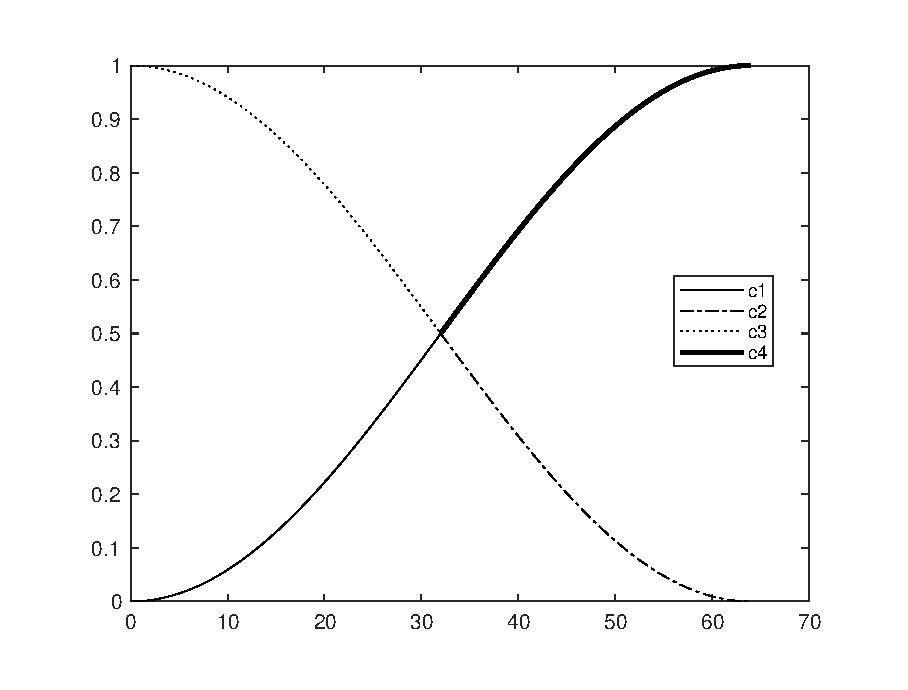
\includegraphics[width=0.95\textwidth]{figure/ex9_41_00.eps}
        \caption*{$\nu_1=0,\nu_2=0$}
    \end{minipage}
    \begin{minipage}[t]{0.32\textwidth}
        \centering
        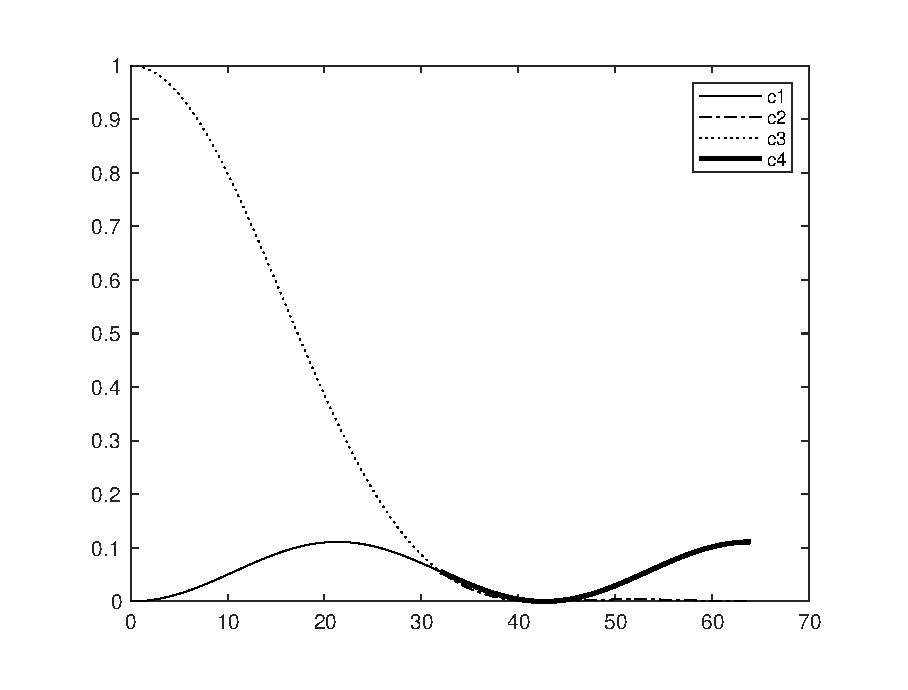
\includegraphics[width=0.95\textwidth]{figure/ex9_41_02.eps}
        \caption*{$\nu_1=0,\nu_2=2$}
    \end{minipage}
    \begin{minipage}[t]{0.32\textwidth}
        \centering
        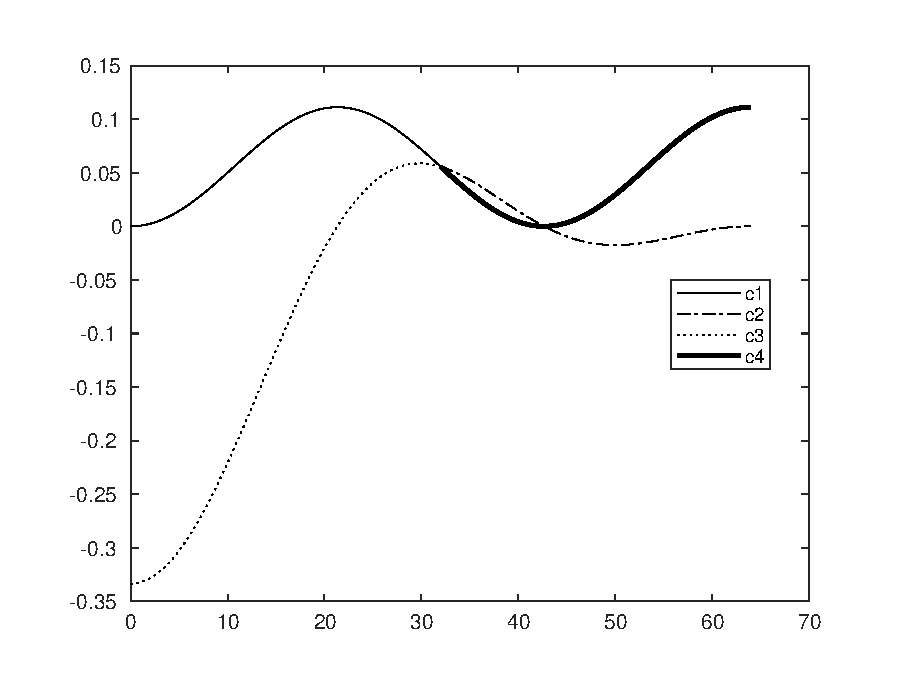
\includegraphics[width=0.95\textwidth]{figure/ex9_41_11.eps}
        \caption*{$\nu_1=1,\nu_2=1$}
    \end{minipage}
\end{figure}
\begin{figure}[H]
    \begin{minipage}[t]{0.32\textwidth}
        \centering
        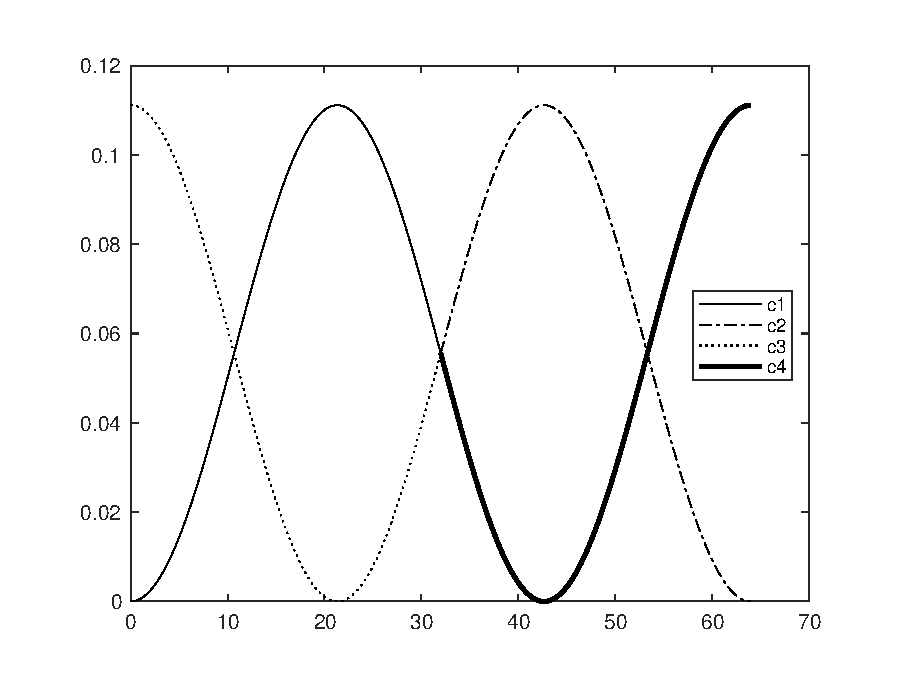
\includegraphics[width=0.95\textwidth]{figure/ex9_41_20.eps}
        \caption*{$\nu_1=2,\nu_2=0$}
    \end{minipage}
    \begin{minipage}[t]{0.32\textwidth}
        \centering
        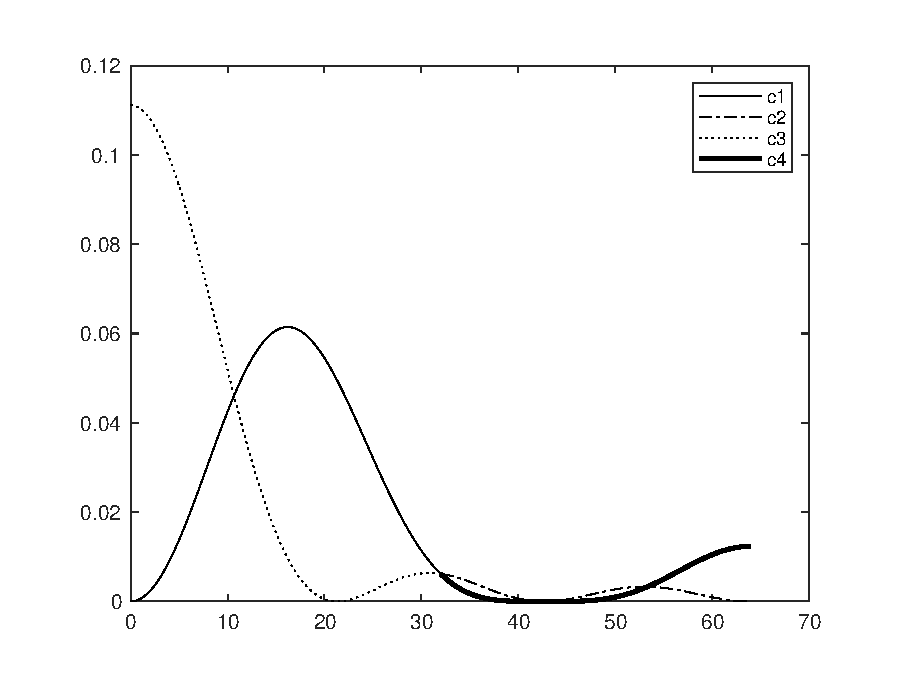
\includegraphics[width=0.95\textwidth]{figure/ex9_41_22.eps}
        \caption*{$\nu_1=2,\nu_2=2$}
    \end{minipage}
    \begin{minipage}[t]{0.32\textwidth}
        \centering
        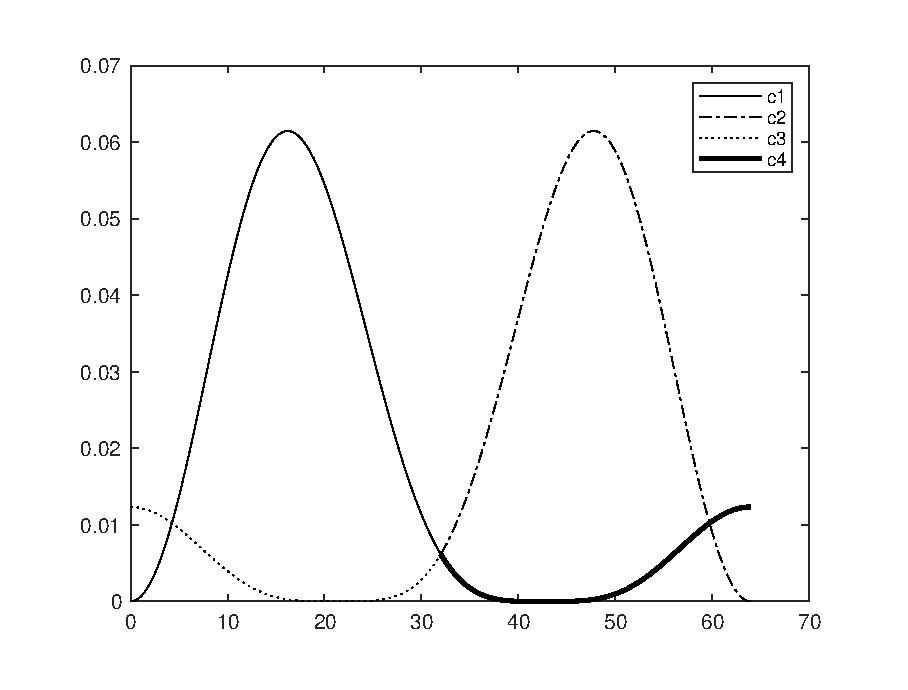
\includegraphics[width=0.95\textwidth]{figure/ex9_41_40.eps}
        \caption*{$\nu_1=4,\nu_2=0$}
    \end{minipage}
    \caption{Reproduce figures in Exercise 9.41.}
\end{figure}

The figures are produced by the following \textbf{matlab} code.
\begin{lstlisting}
    n = 64;
    w = 2/3;
    v1 = 2; v2 = 0;
    lx1 = 0:0.1:n/2; lx2 = n/2:0.1:n;
    y1 = lx1; y4 = lx2; y3 = lx1; y2 = lx2; rho = lx1;
    for lk = 0:5*n
        ind1 = lk+1;
        ind2 = size(lx2,2)-lk;
        k = lk/10;
        lamk = lambda(n,k,w);
        lamk2 = lambda(n,n-k,w);
        sk = (sin(k*pi/(2*n)))^2;
        ck = (cos(k*pi/(2*n)))^2;
        y1(ind1) = lamk^(v1+v2)*sk;
        y4(ind2) = lamk2^(v1+v2)*ck;
        y3(ind1) = lamk2^v1*lamk^v2*ck;
        y2(ind2) = lamk^v1*lamk2^v2*sk;
        T = [y1(ind1),y2(ind2);y3(ind1),y4(ind2)];
        rho(ind1) = max(abs(eig(T)));
    end
    disp([min(rho),max(rho)]);
    plot(lx1,y1,'k')
    hold on
    plot(lx2,y2,'-.k')
    plot(lx1,y3,':k')
    plot(lx2,y4,'k','LineWidth',2)
    legend('c1','c2','c3','c4')

    function lam = lambda(n,k,w)
        lam = 1-2*w*(sin(k*pi/(2*n)))^2;
    end
\end{lstlisting}

The code will also print $\min\rho(\text{TG})$ and $\max\rho(\text{TG})$ for each $\nu_1,\nu_2$. Here are the results.
\begin{table}[H]
    \centering
    \begin{tabular}{cc|cc}
    $\nu_1$        & $\nu_2$         &        $\min\rho(\text{TG})$            &   $\max\rho(\text{TG})$ \\ \hline
    $0$ & $0$ & $1$ & $1$\\
    $0$ & $2$ & $0.1111$ & $0.1111$\\
    $1$ & $1$ & $0.1111$ & $0.1111$\\
    $2$ & $0$ & $0.1111$ & $0.1111$\\
    $2$ & $2$ & $0.0123$ & $0.0617$\\
    $4$ & $0$ & $0.0123$ & $0.0617$
   \end{tabular}
\end{table}

We can see that $\rho(\text{TG})\approx 0.1$ holds for $\nu_1+\nu_2=2$. Moreover, we can reproduce the figures with $n=128$ as following.

\begin{figure}[H]
    \centering
    \begin{minipage}[t]{0.32\textwidth}
        \centering
        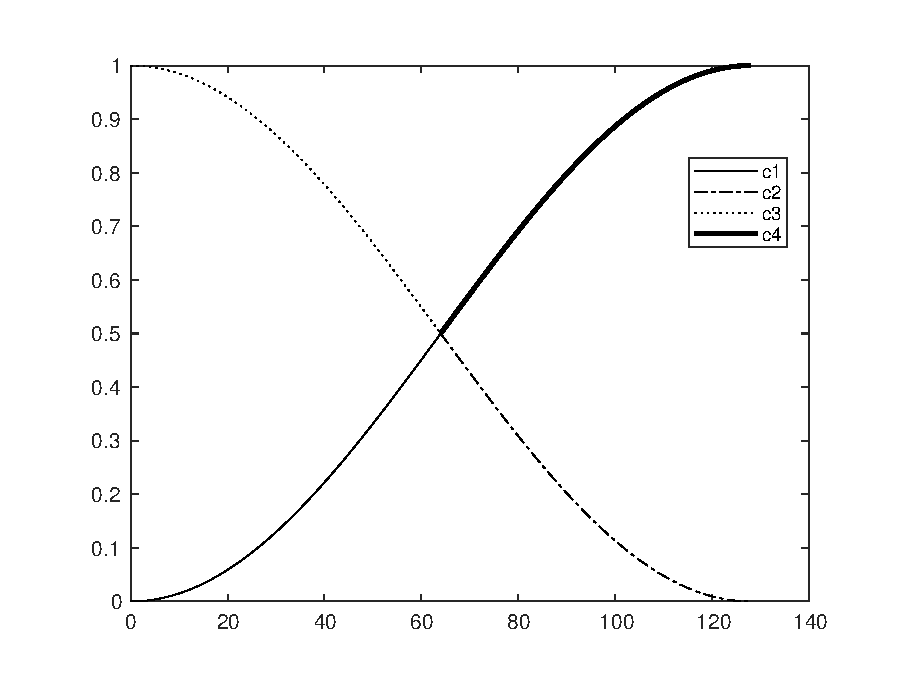
\includegraphics[width=0.95\textwidth]{figure/ex9_41_00_128.eps}
        \caption*{$\nu_1=0,\nu_2=0$}
    \end{minipage}
    \begin{minipage}[t]{0.32\textwidth}
        \centering
        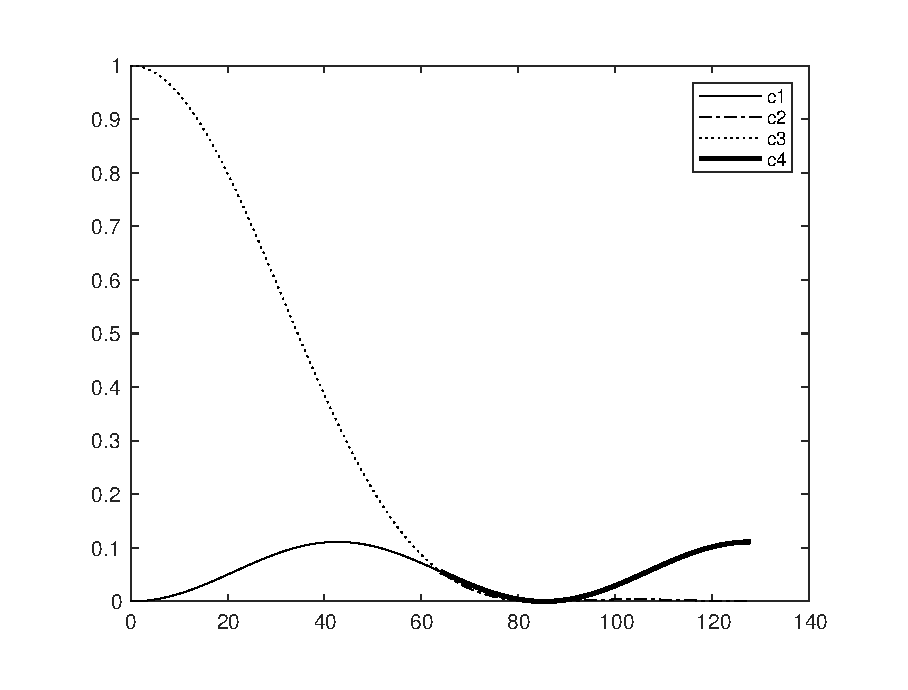
\includegraphics[width=0.95\textwidth]{figure/ex9_41_02_128.eps}
        \caption*{$\nu_1=0,\nu_2=2$}
    \end{minipage}
    \begin{minipage}[t]{0.32\textwidth}
        \centering
        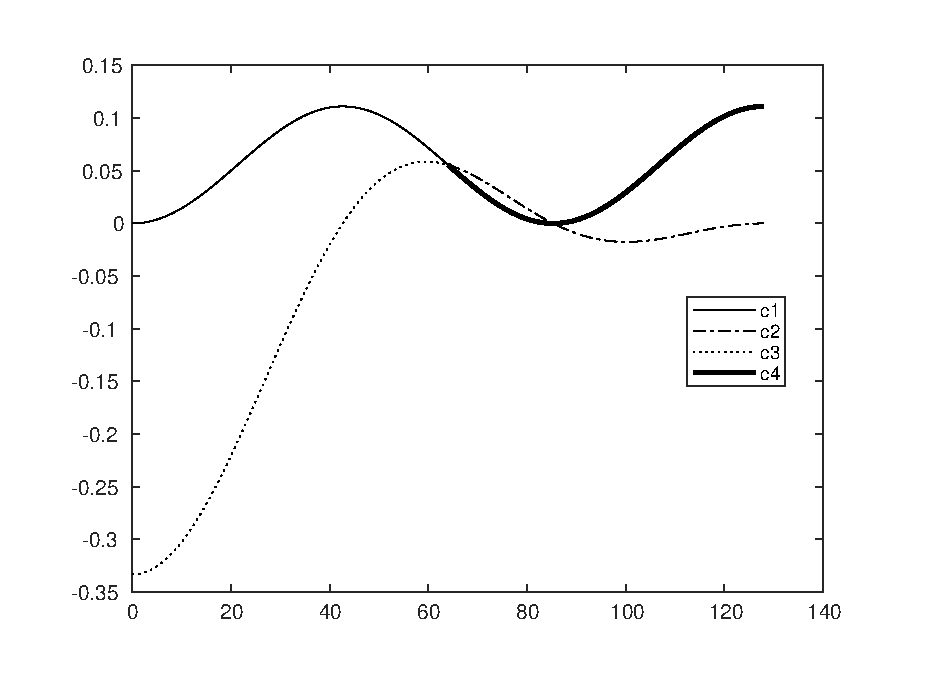
\includegraphics[width=0.95\textwidth]{figure/ex9_41_11_128.eps}
        \caption*{$\nu_1=1,\nu_2=1$}
    \end{minipage}
    \begin{minipage}[t]{0.32\textwidth}
        \centering
        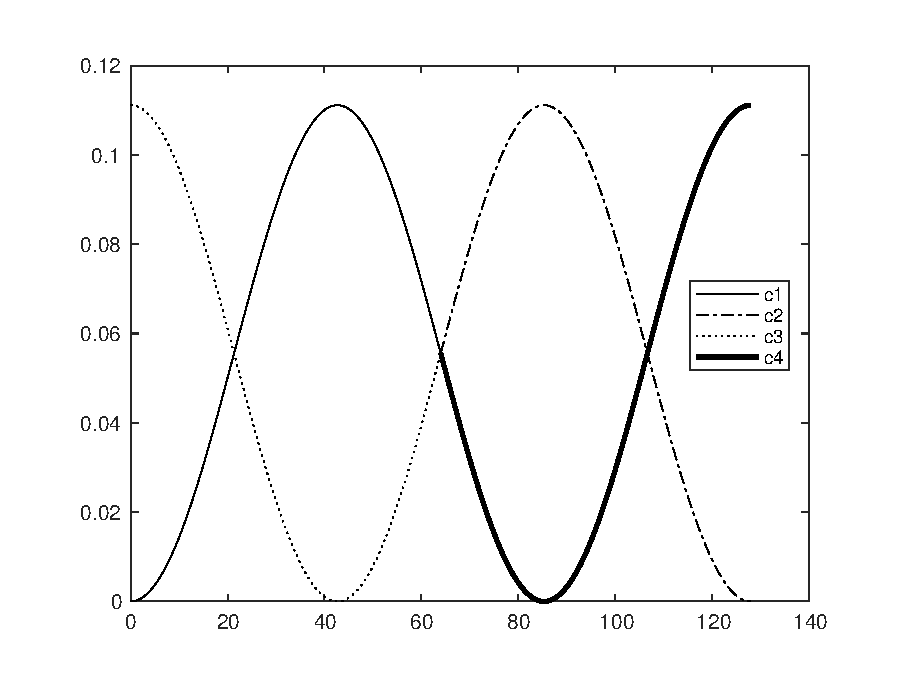
\includegraphics[width=0.95\textwidth]{figure/ex9_41_20_128.eps}
        \caption*{$\nu_1=2,\nu_2=0$}
    \end{minipage}
    \begin{minipage}[t]{0.32\textwidth}
        \centering
        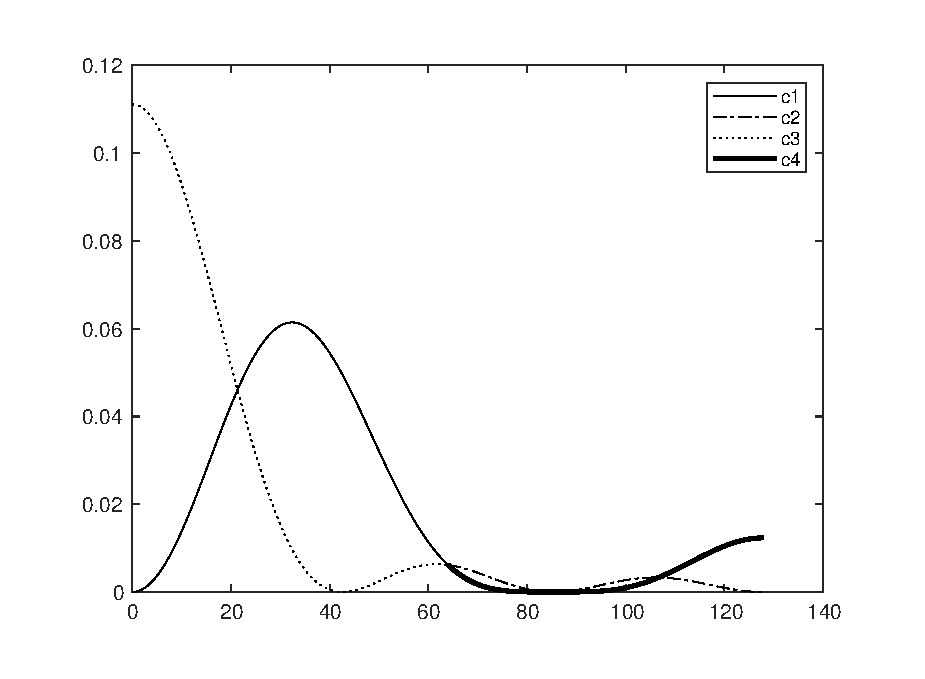
\includegraphics[width=0.95\textwidth]{figure/ex9_41_22_128.eps}
        \caption*{$\nu_1=2,\nu_2=2$}
    \end{minipage}
    \begin{minipage}[t]{0.32\textwidth}
        \centering
        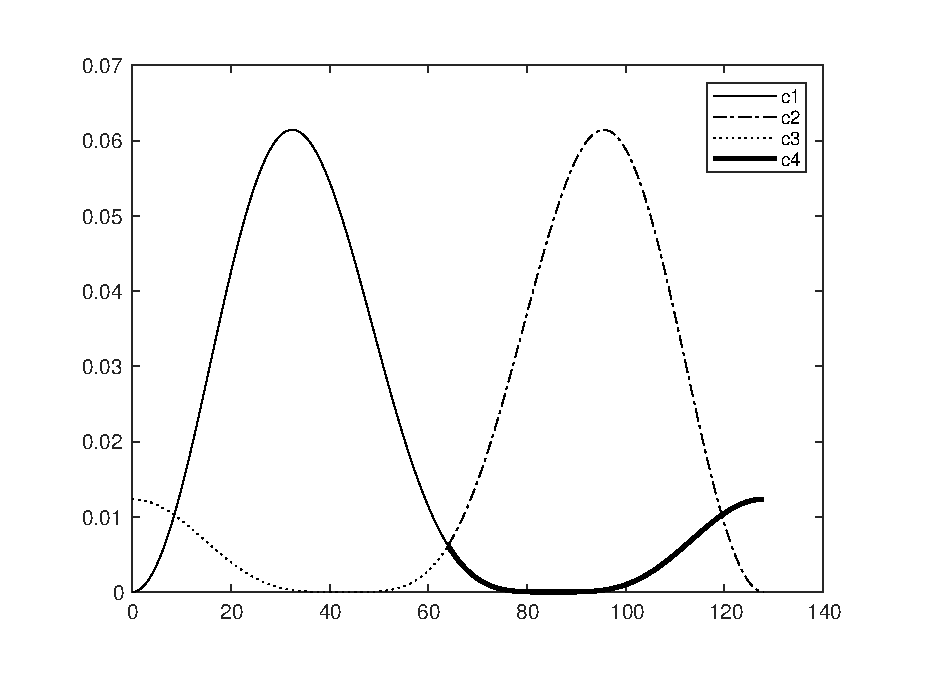
\includegraphics[width=0.95\textwidth]{figure/ex9_41_40_128.eps}
        \caption*{$\nu_1=4,\nu_2=0$}
    \end{minipage}
    \caption{Reproduce figures in Exercise 9.41. for $n=128$}
\end{figure}

We can see the result is independent of the grid size, which implies the independence of $\rho(\text{TG})$ from the grid size.

\section*{X. Exercise 9.45 (Prove Lemma 9.44.)}
\;\;\;\;\;\;By definition 9.25, the full-weighting operator $I_h^{2h}:\mathbb{R}^{n-1}\to\mathbb{R}^{\frac{n}{2}-1}$ is
\begin{equation*}
    I_h^{2h}=\frac{1}{4}\begin{bmatrix}
        1 & 2 & 1\\
        & & 1 & 2 & 1 \\
        & & &  \ddots & \ddots & \ddots \\
        & & &  & 1 & 2 & 1
    \end{bmatrix},
\end{equation*}

which clearly has full row rank. Hence $\text{dim} \mathcal{R}(I_h^{2h})=\frac{n}{2}-1$. By the property of linear map, we have
\begin{equation*}
    \text{dim} \mathcal{N}(T) + \text{dim} \mathcal{R}(T) = \text{dim}(V)\quad \text{for any linear map} \;T:V\to W
\end{equation*}

Hence $\text{dim} \mathcal{N}(I_h^{2h})=n-1-\left(\frac{n}{2}-1\right)=\frac{n}{2}$. That's proved.

\end{document}

%%% Local Variables: 
%%% mode: latex
%%% TeX-master: t
%%% End: 
